\begin{figure}
\centering
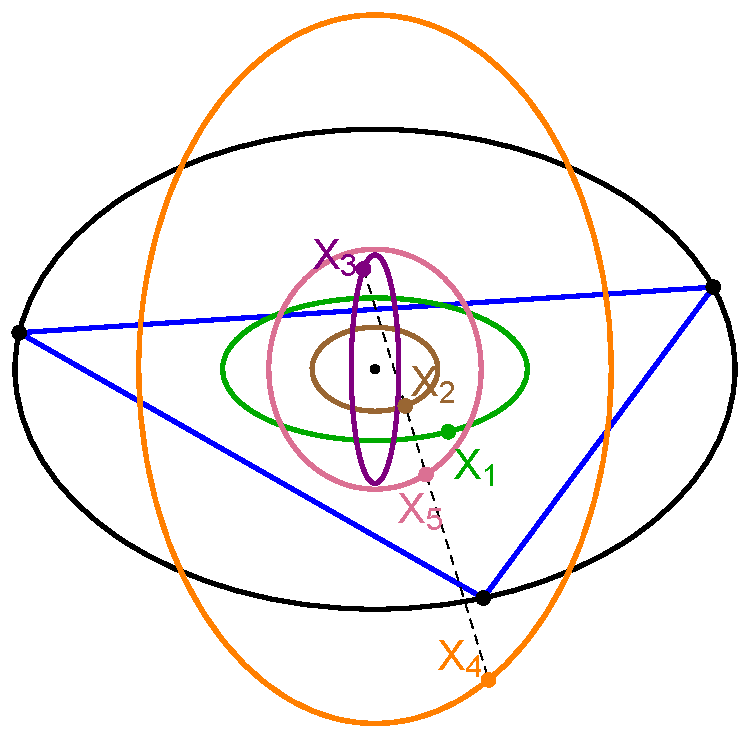
\includegraphics[width=.7\textwidth]{pics_04_060_locus_x12345.pdf}
\caption{Over billiard 3-periodics, the loci of incenter $X_1$, barycenter $X_2$, circumcenter $X_3$, orthocenter $X_4$, and 9-point center $X_5$ are all ellipses. \href{https://youtu.be/sMcNzcYaqtg}{Video}}
\label{fig:04-x12345}
\end{figure}

\begin{figure}
    \centering
    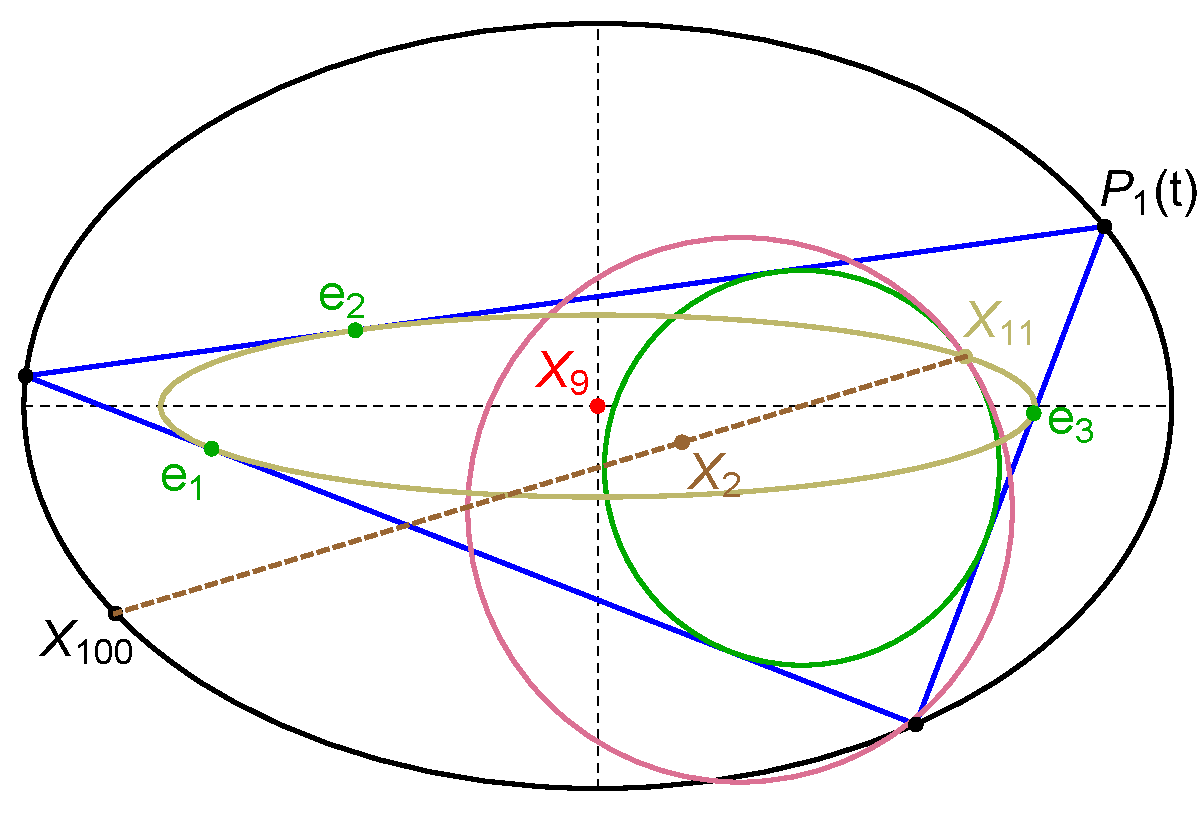
\includegraphics[width=.7\textwidth]{pics_04_080_feuerbach_loci.pdf}
    \caption{A billiard 3-periodic (blue). Also shown are the incircle (green) and 9-point circle (pink) which touch at the Feuerbach point $X_{11}$. Also shown is the latter's {\em anticomplement} $X_{100}$, and the three extouchpoints $e_1,e_2,e_3$. Over the billiard family, $X_{100}$ sweep the billiard while both $X_{11}$ and the extouchpoints sweep the caustic (though in opposite directions).
    % done
    \href{https://youtu.be/TXdg7tUl8lc}{Video}}
    \label{fig:04-feuer-loci}
\end{figure}


\begin{figure}
    \centering
    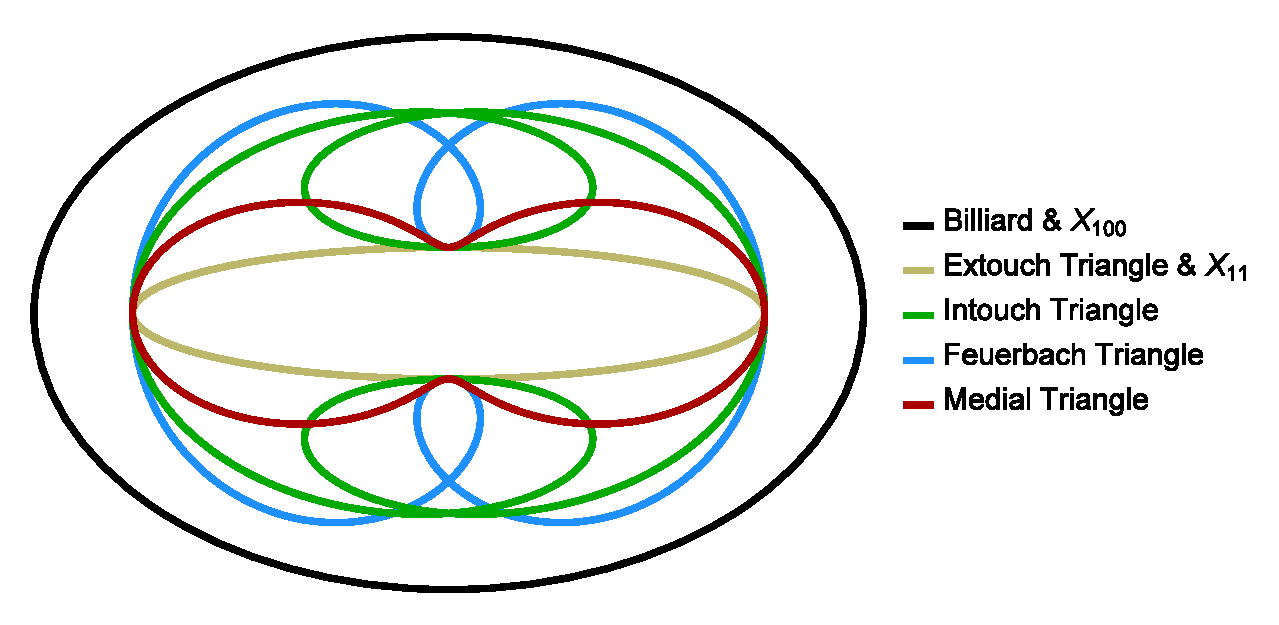
\includegraphics[width=\textwidth]{pics_04_070_non_elliptic.eps}
    \caption{Over billiard 3-periodics, the loci of vertices of certain derived triangles is non-elliptic, namely: the (i) intouch (green), (ii) Feuerbach (not to be confused with the Feuerbach {\em point}) (blue), (iii) medial (red), triangles, and many others not shown. Surprisingly, the vertices of the extouch triangle sweep the confocal caustic (as does the Feuerbach point $X_{11}$, which by definition lies on the Mandart inellipse of any triangle).
     \href{https://youtu.be/OGvCQbYqJyI}{Video}}
    \label{fig:04-non-elliptic}
\end{figure}

\begin{figure}
    \centering
    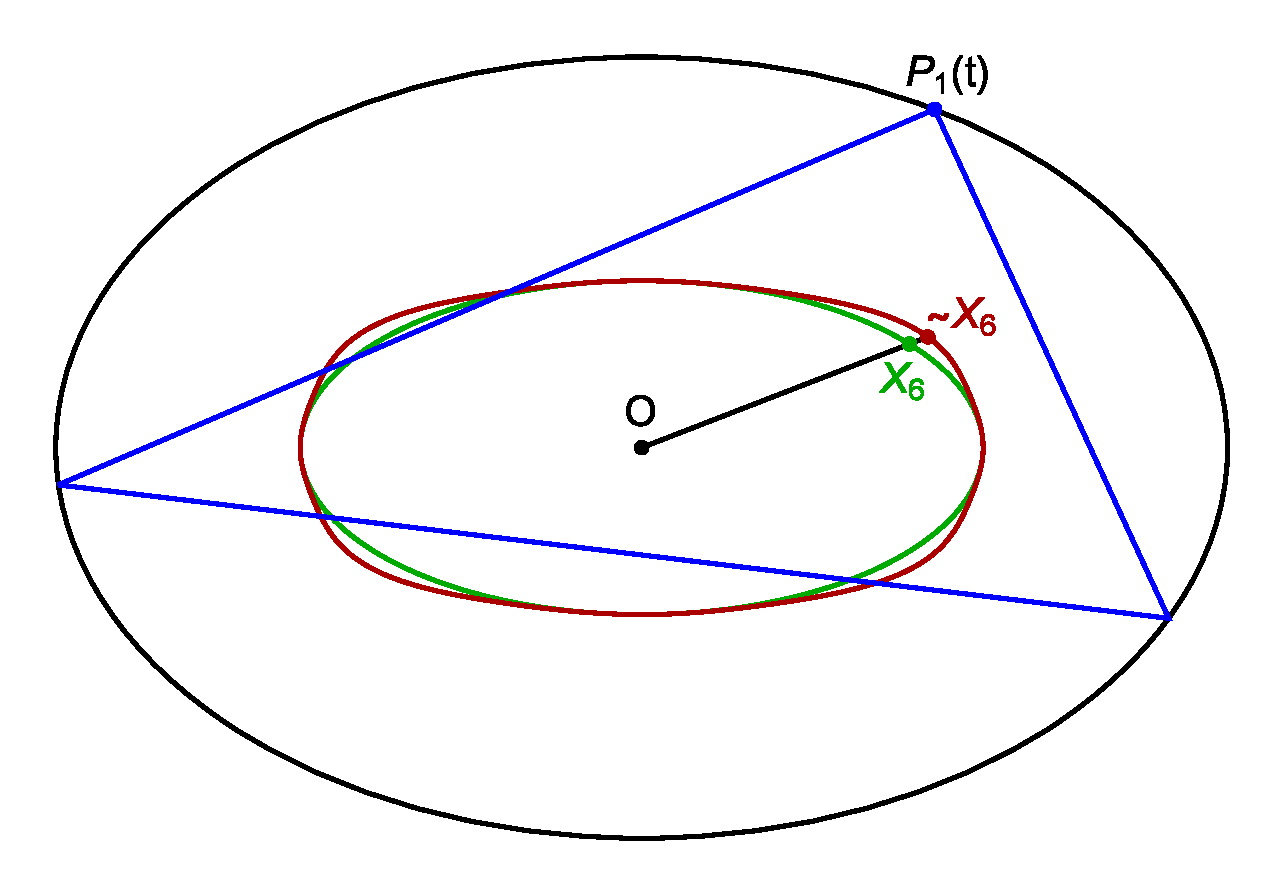
\includegraphics[width=.7\textwidth]{pics_04_090_symmedian.eps}
    \caption{Over billiard 3-periodics (blue), the the locus of the symmedian point $X_6$ (green) is a quartic whose error with respect to the shown ellipse is exaggerated 1000 fold. To the naked eye, the two curves are indistinguishable. \href{https://bit.ly/3qc0Z0L}{app}}
    \label{fig:symmedian}
\end{figure}


\begin{figure}
    \centering
    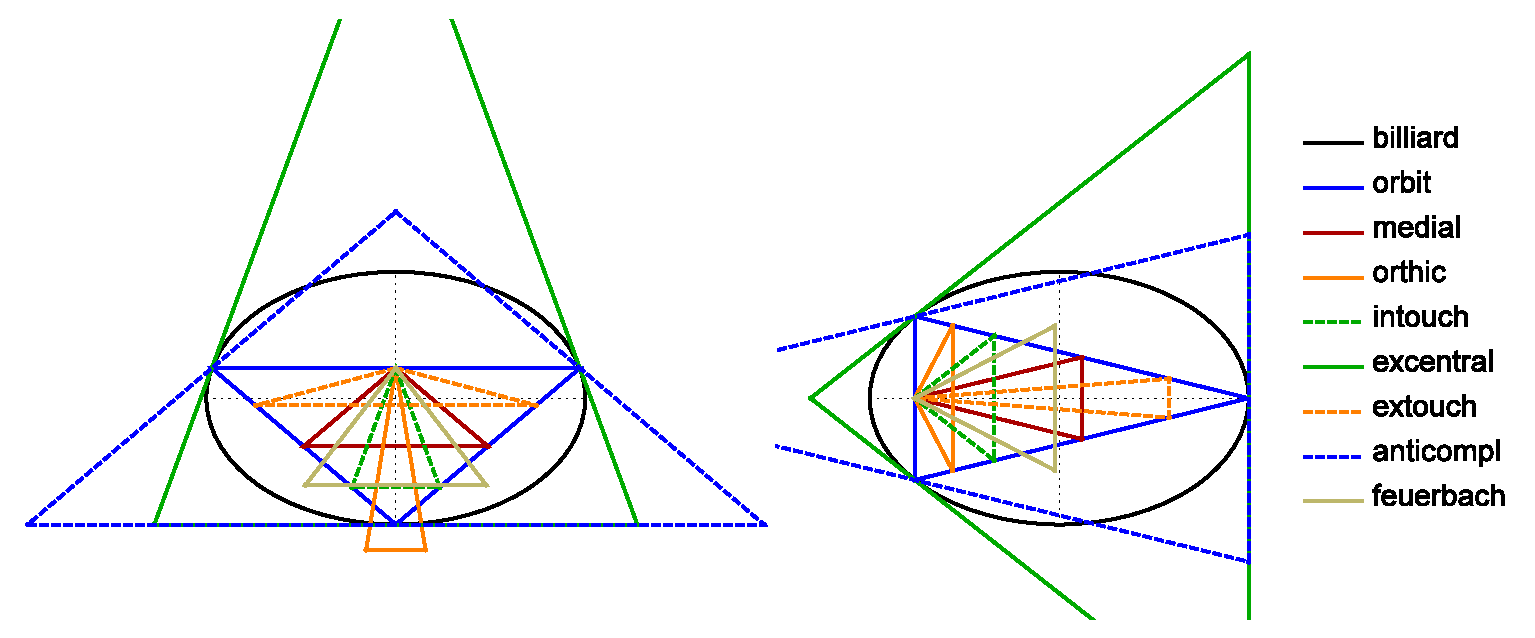
\includegraphics[width=\textwidth]{pics_04_100_confocal_derived.eps}
    \caption{Triangles derived from an isosceles billiard 3-periodic (blue). These contain one vertex on the axis of symmetry. \href{https://youtu.be/xyroRTEVNDc}{Video}}
    \label{fig:04-derived-isosceles}
\end{figure}

% \includegraphics[trim={left bot right upper},clip]
\begin{figure}
    \centering
    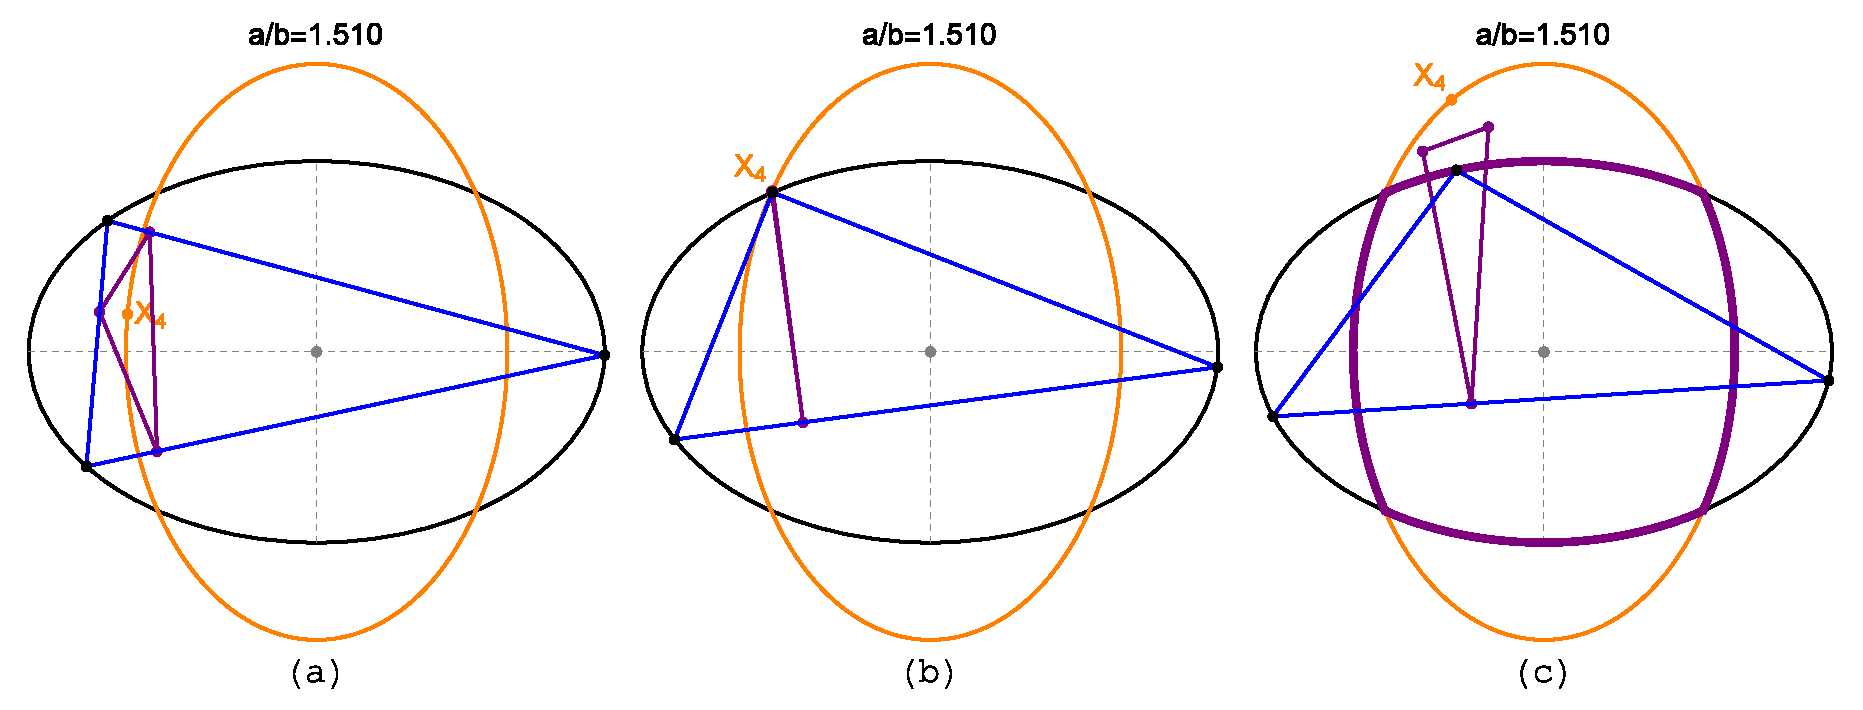
\includegraphics[trim={0 0 0 20},clip,width=\textwidth]{pics_04_120_ort_loci_kink.eps}
    \caption{An $a/b>\alpha_4$ EB is shown (black). Let $T$ and $T_h$ be the 3-periodic and its Orthic Triangle (blue and purple, respectively). \textbf{(a)} $T$ is acute ($X_4$ is interior to the EB), and $I_h=X_4$. \textbf{(b)} $X_4$ is on the EB and $T$ is a right triangle. $T_h$ degenerates to a segment. \textbf{(c)} $X_4$ is exterior to the EB. Two of $T_h$'s vertices are outside $T$. $I_h$ is pinned to $T$'s obtuse vertex, on the EB. $X_4$ is an Excenter of the 3-periodic. The complete locus of $I_h$ comprises therefore 4 elliptic arcs (thick purple) duck-taped at the corners. \href{https://youtu.be/3qJnwpFkUFQ}{Video}, \href{https://bit.ly/33TVjit}{Live}}
    \label{fig:orthic_incenter_locus}
\end{figure}